\documentclass[twocolumn]{IEEEtran}
\usepackage[utf8x]{inputenc}
\usepackage{graphicx}
\usepackage{times}
\usepackage[tbtags]{amsmath}
\usepackage{cite}
%\usepackage{slashbox}
\usepackage{pict2e}
\usepackage{colortbl}
\usepackage{float}
\usepackage[all]{xy}
\usepackage{graphics,graphicx,color,colortbl}
\usepackage{subfigure}
\usepackage{wrapfig}
\usepackage{multicol}
\usepackage{url}
\usepackage[tbtags]{amsmath}
\usepackage{amsmath,amssymb,amsfonts,amsbsy}
\usepackage{bm}
\usepackage{algorithm}
\usepackage{algorithmic}
\usepackage[centerlast, small]{caption}
\usepackage[colorlinks=true, citecolor=blue, linkcolor=blue, urlcolor=blue,
breaklinks=true]{hyperref}

\begin{document}
\title{Lenguaje Ensamblador y la arquitectura MIPS}
\author{David Ricardo Martínez Hernández Código: $261931$\\
	Juan Sebastian Roncancio Arevalo Código: $261585$}
\maketitle
\markboth{Universidad Nacional de Colombia}{}
\floatname{algorithm}{Algoritmo}
\begin{abstract}
  En esta práctica se realizara la implementación del algoritmo de la división en Asembler. Se procedió con el desarrollo explicado en la clase teórica, implementandolo en el lenguaje asembler para obtener la división de dos números enteros positivos.
\end{abstract}
\begin{keywords}
  Asembler, Condicional, División, Lenguaje, Mips, Resta, Suma.
\end{keywords}

\section{Procedimiento}
\noindent
Para cargar un archivo \textit{.s } es necesario tener instalado \textit{QtSpim} y se debe entrar a la interfaz gráfica del programa y hacer lo siguiente:
\begin{enumerate}
 \item Ingresar a File
 \item Entrar a Load File
 \item Cargar el archivo .s que se va a ejecutar
 \item Para ejecutar dicho archivo se ingresa a Simulator
 \item Se hace click en Run$/$Continue o se oprime la tecla F5
\end{enumerate}
\noindent 
EL menú principal de QtSpim tiene las siguientes opciones de menú:
\begin{itemize}
 \item File
 \item Simulator
 \item Register
 \item Text Segment
 \item Data Segment
 \item Window
 \item Help
\end{itemize}

\subsection{Definiciones}
\noindent
El \textbf{proceso de compilación} recibe el lenguaje de más alto nivel lo pasa a un compilador, el cual quita todas las etiquetas que tenga (una etiqueta es una referencia que establece el programador, con un nombre y no con una dirección especifica), luego de pasar al compilador es traducido al lenguaje ensamblador para finalmente enviarlo a un linker, el cual entregara el archivo ejecutable del proceso.\\
Un \textbf{linker} toma todos los objetos junto a las librerías, reservando las direcciones y variables, generando un ejecutable \textit{.s} almacenándolo en memoria.\\
Un \textbf{archivo objeto} es un código máquina que contiene información binaria e información de mantenimiento que ayuda a combinar archivos de un programa.\\
El \textbf{lenguaje ensamblador} es el lenguaje que entienden las máquinas compuesto por $0$ y $1$.\\
La diferencia radica en que el \textbf{lenguaje de alto nivel} esta diseñado para ser comprendido por humanos mientras que el \textbf{lenguaje ensamblador} esta diseñado para las máquinas.\\
Una \textbf{subrutina} es una operación que detiene las instrucciones principales, realiza dicha la operación y continua las operaciones habituales.\\
Una \textbf{interrupción} es una función en la cual detiene la síntesis del programa por completo, hasta que se genere una función que reanude el proceso.

\begin{figure}[H]
	\centering
		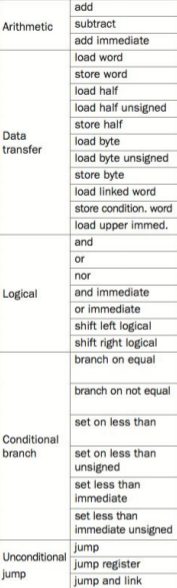
\includegraphics[scale=0.8]{figure.png}
	\caption{Set de instrucciones en lenguaje ensamblador para la arquitectura MIPS32. Tomado de \cite{patterson}, página 78}
	\label{fig2}
\end{figure}


\section{Aplicación}
\noindent
La operación división solo funciona para números positivos enteros, se realiza mediante una serie de restas sucesivas, representado en la Fig. \ref{fig1}

\section{Conclusiones}
\begin{itemize}
 \item Los problemas para realizar este informe fue que nunca se había trabajado en lenguaje  ensamblador y como solo se puede trabajar con dos variables se hizo muy complicado realizar la rutina para la división, se empezó a realizar al suma para recibir los datos  hacer la suma e imprimir el resultado en pantalla, pero generaba un error al realizar al suma, después de solucionar el problema se procedió a hacer la división por medio de las restas sucesivas.
 \item Las operaciones realizadas en el registro aun son desconocidas para nosotros, solo sabemos que se operan pero no sabemos como lo hace, es por eso que no incluimos el signo de los operandos.
 \item Es más sencillo realizar la división por medio de las restas sucesivas, porque solo se tiene que hacer restas hasta que el dividendo sea menor que el divisor.
\end{itemize}

\begin{figure}[H]
	\centering
		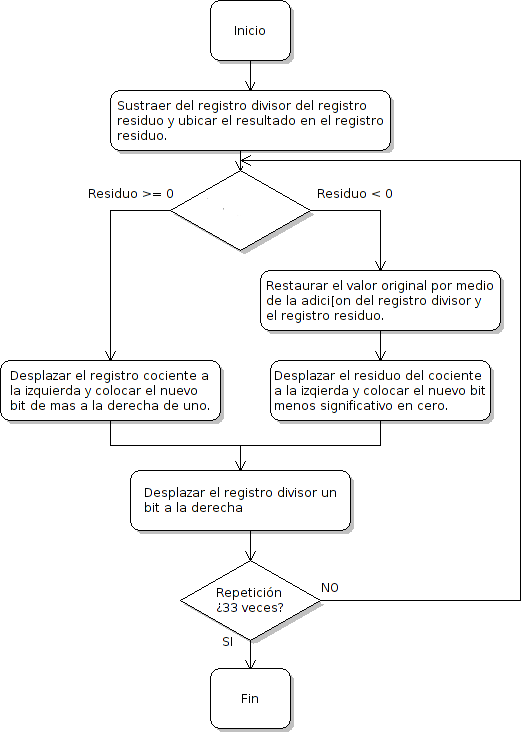
\includegraphics[scale=0.4]{uml.png}
	\caption{Diagrama que se utilizo para realizar la división. Basados en \cite{patterson}, página 238.}
	\label{fig1}
\end{figure}


\bibliographystyle{ieeetran}
\begin{thebibliography}{99}
\bibitem{harris} Harris, David \& Harris, Sarah.
{\em "`Digital desing and computer architecture"'}.
Pretince Hall, 2003.

\bibitem{patterson} Patterson, David \& Hennessy John
{\em "`Computer Organization And Design - The Hardware-Software Interface"'}.
Kindle Edition, Fourth Edition, 2006.

\end{thebibliography}
\end{document}